% vim: tw=80

\chapter{Introduction}

Modern particle physics is driven by the desire to answer the questions about the
fundamental constituents of matter and the principles of interaction between the
constituents. High-energy collisions of particles and the analysis of the
scattering products are a optimal method to gain deep insights into the
fundamental principles of the universe. 

In hadron-hadron collisions at the LHC, point-like parton-parton scattering can
produce outgoing partons with large transverse momenta. The outgoing partons
manifest themselves as a collimated spray of particles, which are clustered into
jets. Events containing two such jets with large transverse momenta, called
dijet events, allow for rigorous tests of perturbative Quantum Chromodynamics
(pQCD) predictions and can subsequently be used to gain a better understanding
of the inner structure of the proton. 

Especially in view of upcoming NNLO corrections for dijet calculations in
perturbative QCD, dijet observables are an optimal candidate for precision
studies of the proton. This lead to the development of the triple-differential
dijet cross section. 

The present thesis presents the analysis of the triple-differential dijet cross
section, which is measured as function of the average transverse momentum of the
two leading jets and binned in the rapidity separation and the boost of the
dijet system. The measurement optimally groups different dijet topologies
according to the underlying momentum fraction of the proton and the scale.


\begin{figure}[h!]
    \centering
    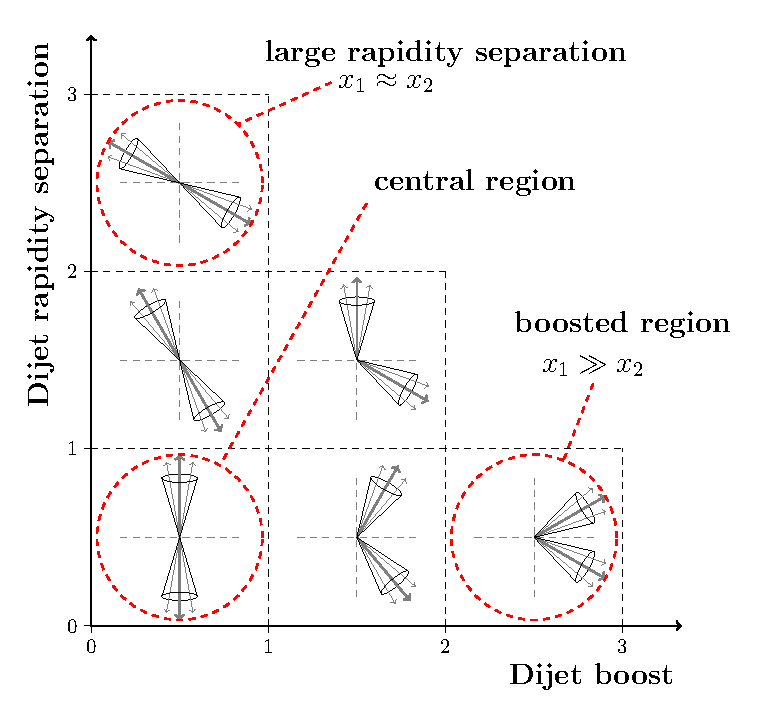
\includegraphics[width=0.4\textwidth]{figures/drawings/ybys_hint.pdf}
\end{figure}

In Chapter~\ref{sec:theoretical_foundations}, the theoretical foundations for
jet production at hadron-hadron colliders are outlined. An overview of the
Standard Model of particle physics with a focus on perturbative quantum
chromodynamics is given. Chapter~\ref{sec:experimental_setup} summarizes the
experimental setup of the LHC collider and the CMS detector. Furthermore, the
employed software tools and Monte Carlo event generators are described. The
reconstruction of jets is detailed in Chapter~\ref{sec:jet_reconstruction}.

The theoretical motivation and the definition of the dijet observables are
introduced in Chapter~\ref{sec:theory_predictions}, in which also the accuracy
of the NLO pQCD calculation is studied. 

The measurement of the triple-differential dijet cross section is explained in
Chapter~\ref{sec:measurement}. The cross section is determined from the data
collected by CMS at \SI{8}{\TeV} which corresponds to an integrated luminosity
of \SI{19.71}{\per \femto \barn}. The measurement is unfolded and compared to
NLO predictions calculated in pQCD.

The sensititivity of the proton PDFs to the measured data is studied in
Chapter~\ref{sec:pdf_constraints} resulting in constraints of the PDFs,
especially the gluon PDF.
